\section{Introduction}

The Interatomic Coulombic Decay (ICD) is an electronic decay process of an atom or
molecule (a unit) involving atoms or molecules of the environment. After an
ionization from the sub-valence region of a unit $A$, the vacancy is filled
by an electron of the same unit and the excess energy is transferred to a decay
partner $B$, which subsequently get ionized:

\begin{equation*}
 A^+ + B \rightarrow A^+ + B^+ + e^-_{ICD}  .
\end{equation*}

The two units $A$ and $B$ are both positively charged, repell each other and
thereby undergo a Coulomb explosion. This process was predicted theoretically
\cite{Cederbaum97} and later proven experimentally \cite{Marburger03}. Since then
it has been studied in a multitude of different systems such as small and large
rare gas clusters \cite{many,Fasshauer14_1},
clusters of small molecules \cite{},
quantum dots \cite{Bande13}
and proteins \cite{Harbach13}. Additionally it has given raise to
the investigation of a whole zoo of ICD-like processes (see Ref. \cite{}
and references therein).

In order to undergo an ICD and it to be observable, two criteria have to
be fulfilled: the energy and the coupling criterion. The energy criterion
requires the energy conservation to hold. In case the doubly ionized final
state is higher in energy than the singly ionized initial state, the ICD
is energetically forbidden. The coupling criterion requires the decay
process to be sufficiently efficient to outperform other decay pathways
such as radiative decay by emission of a photon or coupling to the nuclear
degrees of freedom in molecules. The property calculted for this is the
decay width $\Gamma = \frac{\hbar}{\tau}$, which is inversely proportional
to the lifetime $\tau$ and proportional to the decay rate $\frac{1}{\tau}$.

The ICD process was so far mostly discussed for the case of decay partners in
the direct vicinity, because the decay widths with decay partners further away
was considered to be negligible. Therefore, the decay was studied in clusters
up to 13 neon atoms considering the initial ionization of only the central
atom and not the other ones \cite{Santra01_3}. In this study, a higher than
linear dependence of the decay width on the number of neighbours was
observed. A linear dependence would be expected for equally decay partners
at equal distances from the initially ionized atom in the same environment.
Since the decay width in the asymptotic limit shows an 
$1/\omega^{4}_{vp}$-behaviour on the energy of the virtual photon, which
is decreased for a stabilized final state, this additional feature
can be related to
the better energetic stabilization of the doubly ionized
final state in larger clusters \cite{Fasshauer13}.

We showed that decay pathways with decay partners at larger distances need to
be included for larger systems with many decay partners for two reasons:
\begin{enumerate}
 \item In cluster structures more than one pair of units can consist of
       the same atom types and have the same interatomic distance. Hence,
       they are indistinguishable in the spectrum. Since the decay rate
       is proportional to the number of such pairs as well as the peak
       intensity, the peaks stemming from several pairs are favoured
       compared to other ones at similar distances. Therefore, peaks
       stemming from decays with distant decay partners can be visible
       in ICD spectra of clusters. \cite{Fasshauer14_1}
 \item The opening of ICD-like decay channels depend on the interatomic
       distance. A channel being closed at the distance to the most direct
       beighbours might be open for interaction partners at slightly
       larger distances. If this particular decay channel is more efficient
       than other decay channels being open for the decay with direct
       neighbours, it can still be visible in the spectrum or even
       outperform the slower decay pathways and hence they have to be
       taken into account. We have shown this for the case of ICD vs.
       the Electron Transfer Mediated Decay (ETMD3) process in mixed ArXe
       clusters \cite{Fasshauer13,Fasshauer15_2}.
\end{enumerate}
However, this feature of non-nearest neighbour ICD
has so far not been addressed by itself.

Rare gas clusters are favourable test systems for basic features both
from a theoretical and an experimental point of view. Their spherical
symmetry and their very localized orbitals allow for an comparably easy
theoretical description of the decay processes and the gaseous state
of their components allows for a convenient cleaning of the experimental
setup allowing for higher count rates and therefore a higher resolution
of the spectra. However, the structure of the clusters reveals an
interesting matter of research. Small, ideal clusters exhibit an icosahedral
structure while large clusters have a face-centered-cubic (fcc) structure.
It is still unclear at which cluster size the transition from a favourable
icosahedral to an fcc structure is. Numbers in the range of 800--3000 atoms
have been reported. \cite{}
We propose to use the ICD to be a possible tool to differentiate between
icosahedral and fcc cluster structures using the different distance
patterns in the cluster structures.

We will
therefore first discuss the distance dependency of the ICD in general
in section \ref{sec:theory} and then
zoom in on the NeNe ICD part of the ICD spectra of NeAr clusters
\cite{Fasshauer14_1} in section \ref{sec:near}. Here we will discuss the
peaks and their origin in detail and thereby
raise the question, what a \emph{nearest neighbour} is supposed to be. From
our conclusions we propose the possibility to distinguish cluster structures
of ideal icosahedral and fcc structures using ICD spectra in
section \ref{sec:icofcc}.

%\begin{figure}[h]
% \centering
% \includegraphics[width=\columnwidth]{pics/2dim_coincs.eps}\\
% 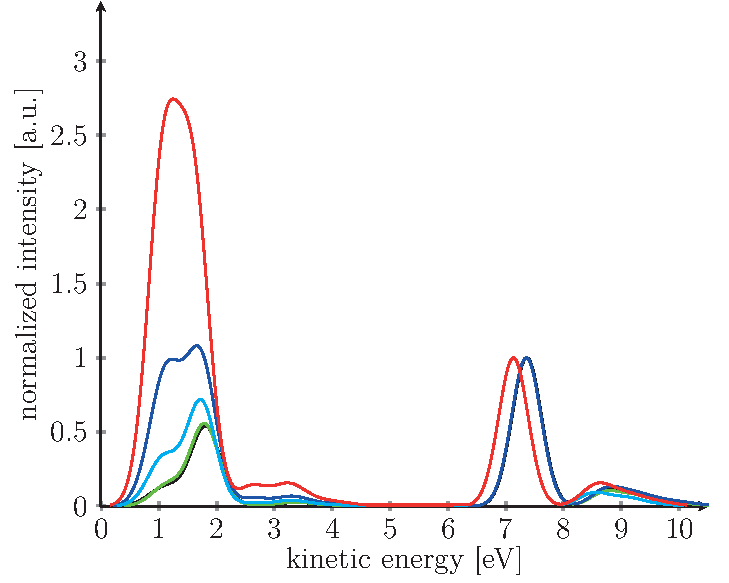
\includegraphics[width=\columnwidth]{pics/NeArcluster_theospecs.pdf}
% \caption{Experimental and theoretical NeAr ICD spectra \cite{Fasshauer14_1}.
%          The experimental spectra were obtained for different cluster expansion
%          conditions and the theoretical spectra were obtained for different
%          underlying cluster structures. In both the NeNe and the NeAr ICD part
%          of the spectrum a main peak and next to it at least one more peak at
%          higher energies are observed. These smaller peaks stem from decays
%          with decay partners at larger distances \cite{Fasshauer13,Fasshauer14_1}.}
% \label{figure:near_spectra}
%\end{figure}
